\chapter{Pen, fingers, the Draw tab, papers, the board and VR}
\label{ch:pen}

\section{Fingers and a pen on a 2-in-1}
Tablet Mode (the tab menu, or Preferences $>$ Pen and touch: Auto follows the laptop's fold) makes the targets half as
big again (7~mm for a pen), and then fingers navigate while the pen works: one finger drags to orbit (a flick glides
on), taps to select, double-taps to frame; two fingers pinch to zoom, drag to pan, twist to turn; one finger scrolls a
list; the pen selects, moves, draws and paints, its side button held orbits (\key{Shift} pans, \key{Ctrl} zooms), its
side button clicked, or the pen or a finger held still half a second, opens \textbf{the Wheel}: one radial menu with
Undo, Delete, Extrude, the brushes, sizes and symmetry of whatever mode you are in; right-click any menu row $>$ \ui{Add
to the Wheel} puts a command on it. A finger's press waits a moment before it counts, so a pinch never starts a box
select; a palm resting on the screen while the pen is near is ignored. On Linux fingers and pens come through XInput 2;
on a Mac the trackpad's pinch and twist navigate and a tablet's pen has its pressure and tilt. The pen's pressure drives
the sculpt and paint brushes (a Pressure Curve in the brush settings), its tilt turns Flatten's and Scrape's plane and
widens a drawing brush, its eraser end erases and inverts.

\section{A pen display's dial and express keys}
Pen displays such as XPPen's send their express keys as keyboard shortcuts and their dial as a key pair or the wheel;
Blendity answers them where the pen draws: \key{Ctrl -} / \key{Ctrl =} zoom about the pen, \key{[} / \key{]} the brush
size, \key{4} / \key{6} turn the canvas and \key{5} sets it upright (Krita's keys \cite{Krita2026}), \key{B} brush,
\key{E} eraser, \key{Space} held pans, \key{Ctrl 0} fits; \ui{More > Wheel / Dial} chooses what the wheel does.

\section{The Draw tab}
\menu{Window > Draw} is the pad: the scene from the Scene or the Game camera, or blank Paper, the pen drawing in that
perspective while the keyboard moves the view (the arrows, \key{A} / \key{D}, \key{W} / \key{S} orbit and dolly the
camera while the pen is up), every stroke placed in the scene where it was drawn. It works like SketchBook Pro's canvas
\cite{SketchBookDocs2026}: one slim toolbar (Undo, Redo, Brush, the color with its opacity, Size, Ruler, Ellipse,
Curve, Symmetry, Perspective, Steady Stroke, Predictive Stroke, Layers, the zoom and More), the pad zoomed, panned,
turned and flipped with the wheel, a middle-drag or \key{Space}+drag and two fingers, \key{Tab} to hide the tools. The
brush palette holds Pencil, Pen, Inker, Felt Pen, Marker, Airbrush and two erasers, with the puck (drag sideways for
the size, up and down for the opacity; \key{B} held and dragged puts it at the pen) and Brush Properties on a
double-click. The \textbf{Layers} window composites the sketch's layers as Photoshop does \cite{PhotoshopHelp2026}:
opacity, the 27 blend modes, groups, locks, Clip to the layer below, a layer mask from a selection; \ui{More > Select}
has rectangle and lasso selections (\key{Alt+Backspace} fills, \key{Delete} cuts, \key{Ctrl+D} deselects) and \key{Ctrl+T}
Free Transform; \ui{More > Shapes} has Rectangle, Ellipse, Polygon, Star and Illustrator's Pen with fills, artboards
and SVG in and out. \ui{Place in 3D} puts each stroke in the scene at the depth under the pen; \ui{Build} and \ui{Lift}
make geometry from the construction lines (chapter~\ref{ch:plan}).

\begin{figure}[H]
  \centering
  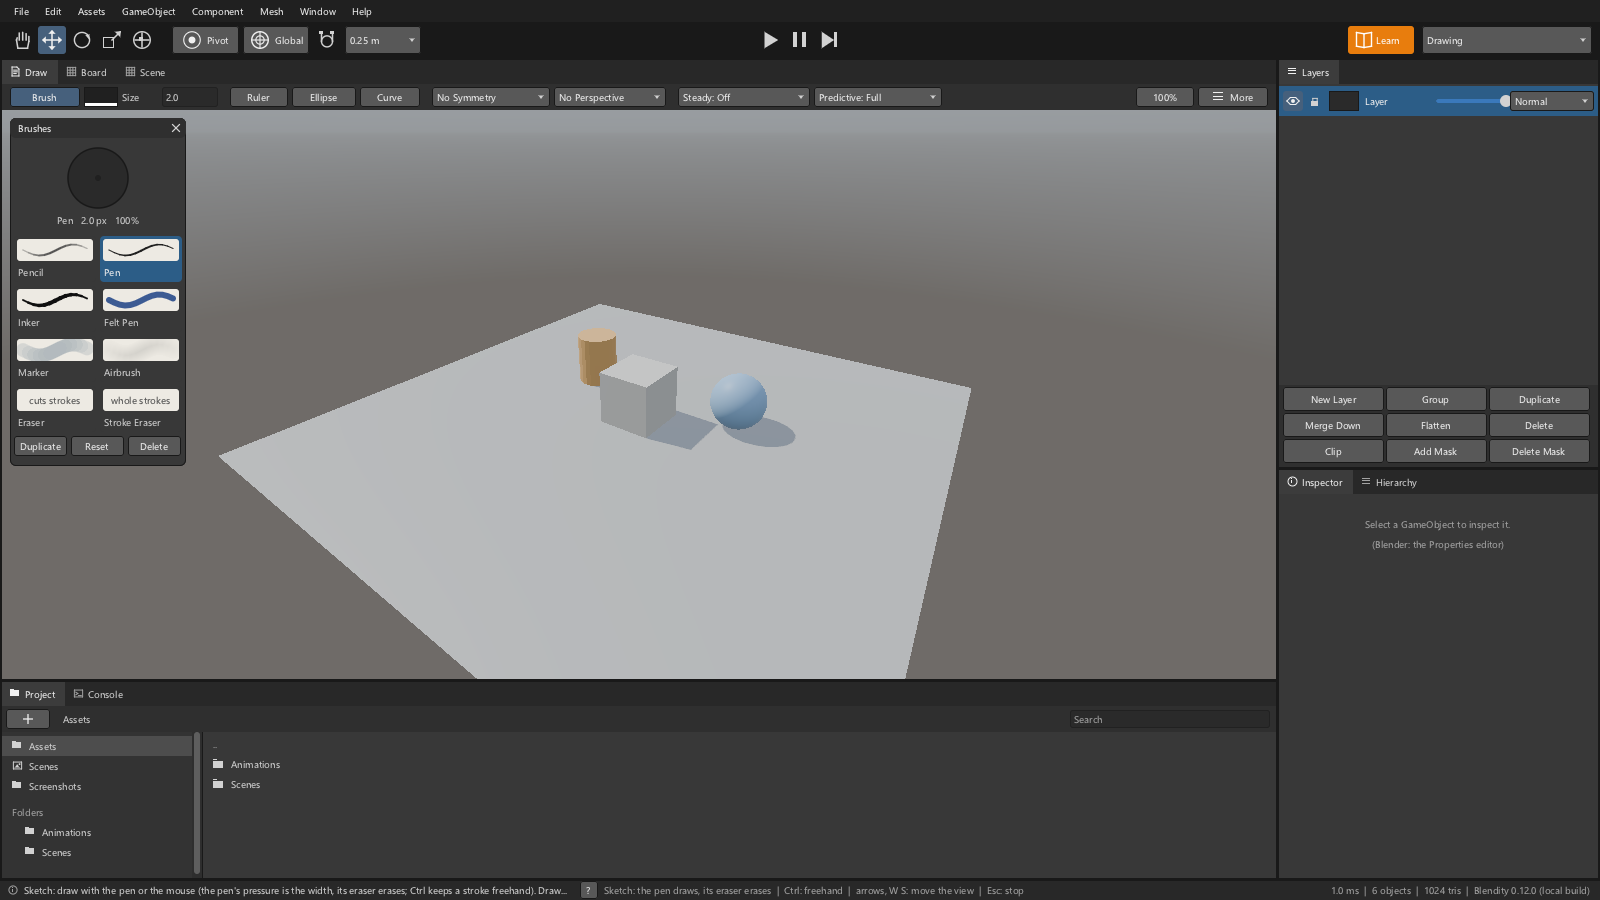
\includegraphics[width=\textwidth, alt={The Drawing layout: the Draw tab's pad with its slim toolbar at the top, the Layers window and the Project window.}]{layout-drawing.png}
  \caption{The Drawing layout: the Draw tab's pad with its toolbar, the Layers window and the Project window.}
\end{figure}

\section{Papers}
\ui{More > Source > Paper} draws on a paper: a page of its own in \code{Assets/Papers}, not in the scene. \ui{New Paper},
\ui{Open Paper}, \ui{Duplicate} and \ui{Delete} live under \ui{More > Paper}; a paper saves itself a second after each
change and on closing, and the one used last opens again. A paper can be pinned to the board, where double-clicking it
draws on it.

\section{The board}
\menu{Window > Board} is a PureRef-style reference board \cite{PureRef2026}: drop images from the system, drag them from
the Project window, \ui{Add Image\ldots} or \key{Ctrl+V} a screenshot; the wheel zooms about the pointer, a middle-drag
pans, \key{Home} fits everything, \key{F} frames the selection; drag to move, a corner to scale, the round handle to turn
(\key{Ctrl}: 15-degree steps); \key{Ctrl+]} / \key{Ctrl+[} to the front and back, \key{Ctrl+D} duplicates, \key{Delete}
removes; its own undo history; it saves itself to \code{Assets/Boards} and opens again next time; \menu{Boards >
Export\ldots} writes PNG, JPEG or PDF.

\section{VR View}
\menu{Edit > VR View} (\code{vr start}) shows the scene in an OpenXR headset (SteamVR, Quest Link, Windows Mixed
Reality \cite{OpenXR2026}) at life size, standing on the ground below where the Scene view looks. Squeeze a grip and
drag to move the world; both grips to scale or turn it; hold the right trigger to throw a teleport arc; the left stick
walks, the right snap-turns; \key{A} shows a tape measure. \code{vr sketch on}: the right trigger draws ribbons or tubes
in the air with pressure and a palette, into a Stroke object that renders and exports like any mesh. \code{vr paint
on}: paint the object with the desk's brush where the controller's ray meets it. It needs the build with Blender's
libraries, on Windows.

\begin{fromnote}{Learn}
\emph{The Editor Layout > Fingers and a pen on a 2-in-1}, \emph{Customizing the Editor}, \emph{Drawing like SketchBook},
\emph{Papers}, \emph{Drawing in Perspective}.
\end{fromnote}
